\documentclass[letterpaper,11pt]{article}

\usepackage[spanish,english]{babel}
\usepackage[top=2cm,bottom=2cm,right=2cm,left=2cm]{geometry}
\usepackage{circuitikz}
\usepackage{amssymb}
\usepackage{amsmath}
\usepackage{amsthm}
\usepackage{mathrsfs}
\usepackage{empheq}
\usepackage{emptypage}
\usepackage{mdframed}
\usepackage{booktabs}
\usepackage{lipsum}
\usepackage{graphicx}
\usepackage{color}
\usepackage{psfrag}
\usepackage{pgfplots}
\usepackage{bm}
\usepackage{multicol}
\usepackage{wrapfig}
\usepackage{float}
\usepackage{fancyhdr}
\usepackage{wrapfig}
\usepackage{multirow}
\usepackage{csquotes}
\usepackage{parskip}
\usepackage{cancel}
\usepackage{listing}
\usepackage{tikz}
\usepackage{verbatim}
\usepackage{subcaption}
\usepackage{enumitem}
\usepackage{xcolor}
\usepackage{xfrac}
\usepackage{hyperref}

\graphicspath{{fig/}}
%\addbibresource{biblio.bib}
\usepgfplotslibrary{colorbrewer}
\pgfplotsset{width=8cm,compat=1.9}
\definecolor{negro}{RGB}{0,0,0}
\definecolor{azul}{RGB}{0,0,255}
\definecolor{verde}{RGB}{0,255,0}
\definecolor{cian}{RGB}{0,255,255}
\definecolor{rojo}{RGB}{255,0,0}
\definecolor{magenta}{RGB}{255,0,255}
\definecolor{amarillo}{RGB}{255,255,0}
\definecolor{blanco}{RGB}{255,255,255}

\definecolor{limegreen}{cmyk}{0.75,0,1,0}
\definecolor{orange}{cmyk}{0,0.8,0.95,0}
\definecolor{purple}{cmyk}{0.75,1,0,0}
\begin{document}
\begin{center}
    \vspace{12mm}

    \LARGE{\textit{Fluido  Lennard–Jones \\ en dos dimensiones}}
    \vspace{3mm}
    
    \textit{\large{Fajardo Fernando, Ospina Juan P.}}
    \vspace{1mm}
            
    \normalsize{12 de Octubre, 2026}
    \vspace{10mm}
\end{center}

\vspace{35pt}

\Large


\begin{center}

    \textbf{Resumen}
    
        Se analiza el fluido bidimensional con potencial de Leonnard-Jones mediante métodos como Verlet-Velocity usando 36 partículas dentro de una caja con $\ell = 12$ y usando unidades naturales para $\sigma$ y $\epsilon$ ---Ambas tomando el valor de 1---; por otra parte, se usó el algoritmo mt19937 correspondiente al algoritmo Mersenne Twister que tiene un periodo de $2^{19937}-1$ para la generación de las posiciones y velocidades tanto en $x$ como en $y$ para cada una de sus partículas.
    
    \vspace{10pt}
     
        \textbf{Palabras clave} --- \textit{}
    
    \vspace{25pt}
     
\end{center}

\begin{multicols}{2}

\section*{Introducción}

    El modelo estándar para simular sistemas moleculares y atómicos bidimensionales es el Fluido Lennard-Jones, el cual describe de forma aproximada pero robusta las interacciones de van der Waals entre átomos neutros o moléculas esféricas. Mediante simulaciones de Dinámica Molecular (MD) o Monte Carlo (MC), es posible rastrear las trayectorias microscópicas para calcular observables macroscópicos y estructurales tales como la energía cinética ($K$), energía potencial ($U$), energía total ($E$), coeficientes de difusión y cambios estructurales inducidos por la densidad o la energía.

    


\section*{Marco Teórico}

    Partiendo del Hamiltoniano del sistema:

    \begin{align*}
        H = \sum_{i=1}^{N} \frac{1}{2} m |\mathbf{v}_i|^2 + \sum_{i<j} U\big(|\mathbf{r}_i - \mathbf{r}_j|\big)
    \end{align*}

    Se plantea la fuerza sobre cada partícula como el gradiente negativo del potencial $\mathbf{F}_{ij} = -\nabla U(r_{ij})$; y se deriva el potencial de Lennard-Jones

    \begin{align*}
        \mathbf{F}_{ij} = \frac{24 \epsilon}{r_{ij}^2} \Bigg[ 2\Bigg(\frac{\sigma}{r_{ij}}\Bigg)^{12} - \Bigg(\frac{\sigma}{r_{ij}}\Bigg)^{6} \Bigg] \mathbf{r}_{ij}
    \end{align*}

    Donde $\mathbf{r}_{ij}$ se calcula de la forma:

    $\Delta x = x_i - x_j - l \cdot \text{round}\big[(x_i - x_j)/l\big]$

    Y aplicando la segunda ley de Newton con la reducción de orden ---$\dot{\mathbf{r}} = \mathbf{v}$--- se obtiene el sistema:

    \begin{align*}
        \dot{\mathbf{r}}_i = \mathbf{v}_i \; \; , \hspace{10pt} \dot{\mathbf{v}}_i = \mathbf{a}_i = \frac{1}{m}\sum_{j \neq i} \mathbf{F}_{ij}
    \end{align*}

    Donde $\mathbf{a}_i$ se le conoce como la aceleración de la partícula $i$; por lo que se puede usar el método de Velocity-Verlet tomando la forma:

    \begin{equation*}
        \mathbf{r}_{n+1} = \mathbf{r}_n + \mathbf{v}_n \Delta t + \frac{1}{2}\mathbf{a}_n \Delta t^2
    \end{equation*}

    Y calculando la nueva aceleración $\mathbf{a}_{n+1} = \mathbf{a}(\mathbf{r}_{n+1})$, se actualiza la velocidad:

    \begin{align*}
        \mathbf{v}_{n+1} &= \mathbf{v}_n + \frac{1}{2}\big(\mathbf{a}_n + \mathbf{a}_{n+1}\big)\Delta t
    \end{align*}

    Por último, a partir de las trayectorias se definen los observables; la función de distribución radial, que mide la probabilidad de encontrar una partícula a distancia $r$ de otra relativa a un gas ideal:

    \begin{align*}
        g(r) = \frac{l^2}{N^2} \frac{\langle n(r) \rangle}{2 \pi r \, \Delta r}
    \end{align*}

    Y el desplazamiento cuadrático medio, cuyo régimen lineal permite obtener el coeficiente de difusión en dos dimensiones:

    \begin{align*}
        \text{MSD}(t) &= \frac{1}{N}\sum_{i=1}^{N} |\mathbf{r}_i(t) - \mathbf{r}_i(0)|^2 \\ \text{MSD}(t) &\approx 4Dt
    \end{align*}

\section*{Resultados y Conclusiones}

    El fluido de Lennard-Jones, como se muestra en la figura 1, se inicializó con $N = 36$ partículas en una caja de lado $l = 12$ ---densidad $\rho = N/l^2 = 0.25$--- con $\epsilon = \sigma = 1$, cuyas posiciones y velocidades se generaron mediante el algoritmo pseudoaleatorio $mt19937$ nativo de C++ con semilla fija $654321$ para la elección de números dentro de una distribución uniforme.

    \begin{figure}[H]
        \centering
        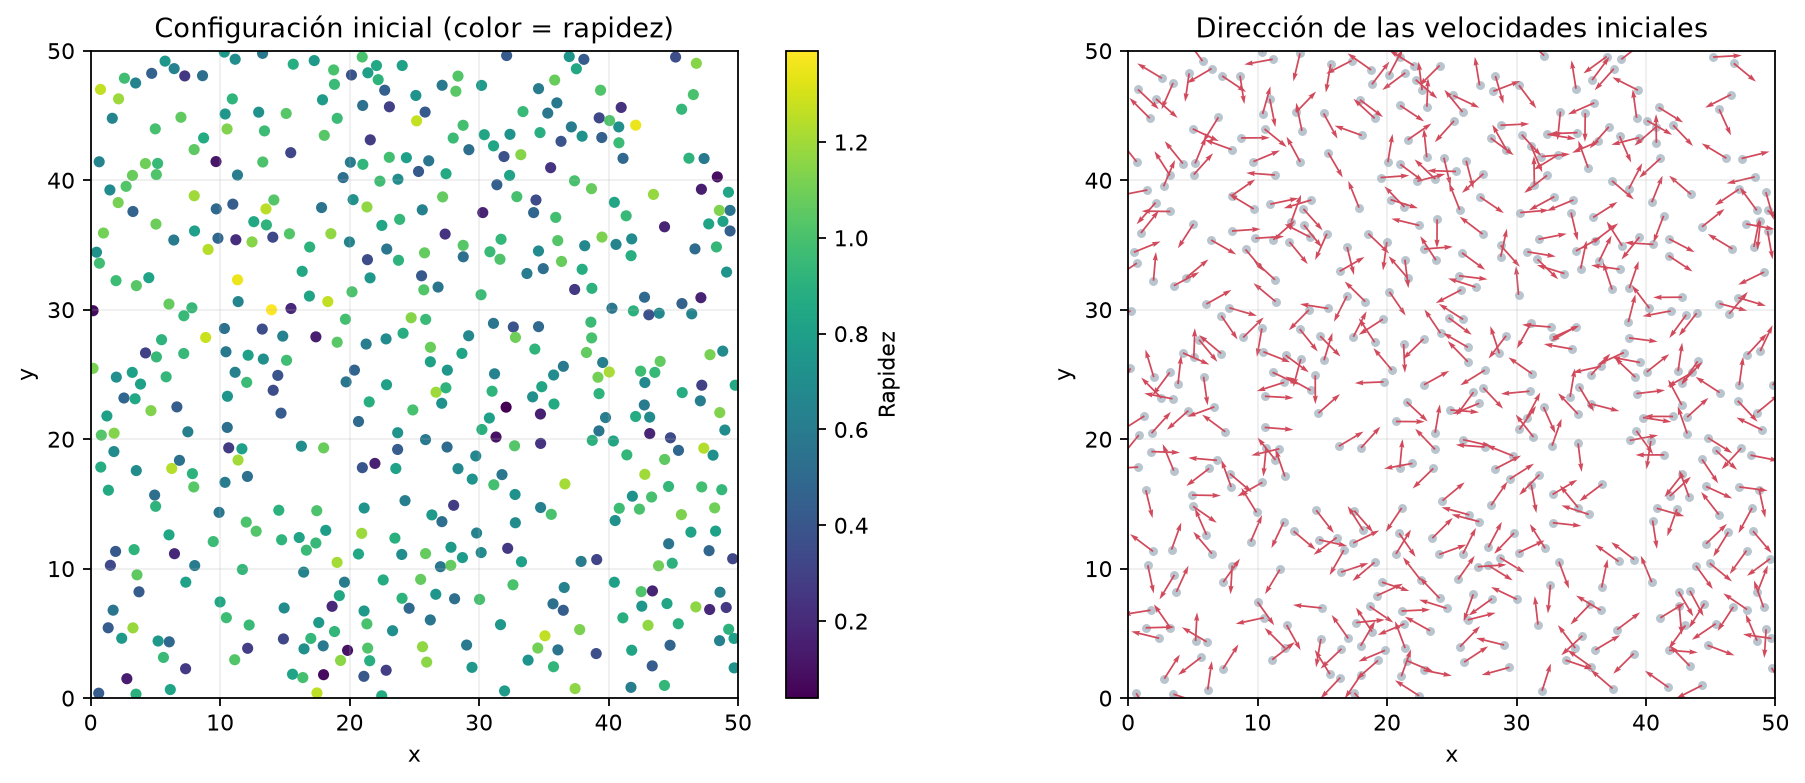
\includegraphics[width=0.9\linewidth]{configuracion_y_velocidades.png}
        \caption{Configuración inicial de posiciones y velocidades de las $N = 36$ partículas del fluido de Lennard-Jones.}
    \end{figure}

    Tras la integración mediante el método de Velocity-Verlet con $\Delta t = 0.001$ hasta $t_f = 10$ ---$10^4$ pasos--- como se puede ver en la figura 2, el Hamiltoniano pasó de $H_{\text{ini}} = 26.5694$ a $H_{\text{fin}} = 26.5578$, es decir, una variación relativa $\Delta H / H \approx 4.4 \times 10^{-4}$.

    \begin{figure}[H]
        \centering
        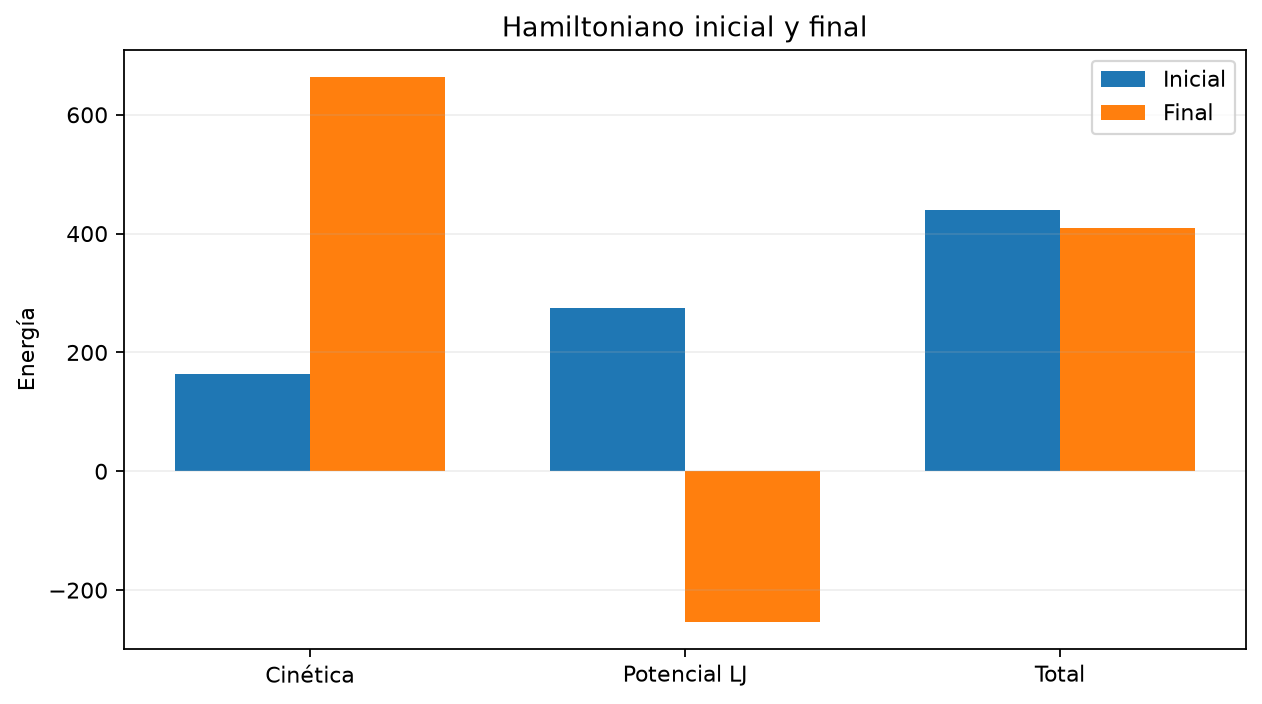
\includegraphics[width=0.9\linewidth]{hamiltoniano_inicial_final.png}
        \caption{Comparación del Hamiltoniano inicial y final del fluido de Lennard-Jones mediante el método de Velocity-Verlet.}
    \end{figure}

    Por otra parte, la función de distribución radial ---figura 3--- presentó su pico principal en $r \approx 1.125$ con $g(r) \approx 1.67$, el cual coincide con el mínimo del pozo de potencial $r_{\min} = 2^{1/6}\sigma \approx 1.12$, y para distancias grandes tiende a $g(r) \approx 1$, que es lo esperado para un fluido sin orden de largo alcance.

    \begin{figure}[H]
        \centering
        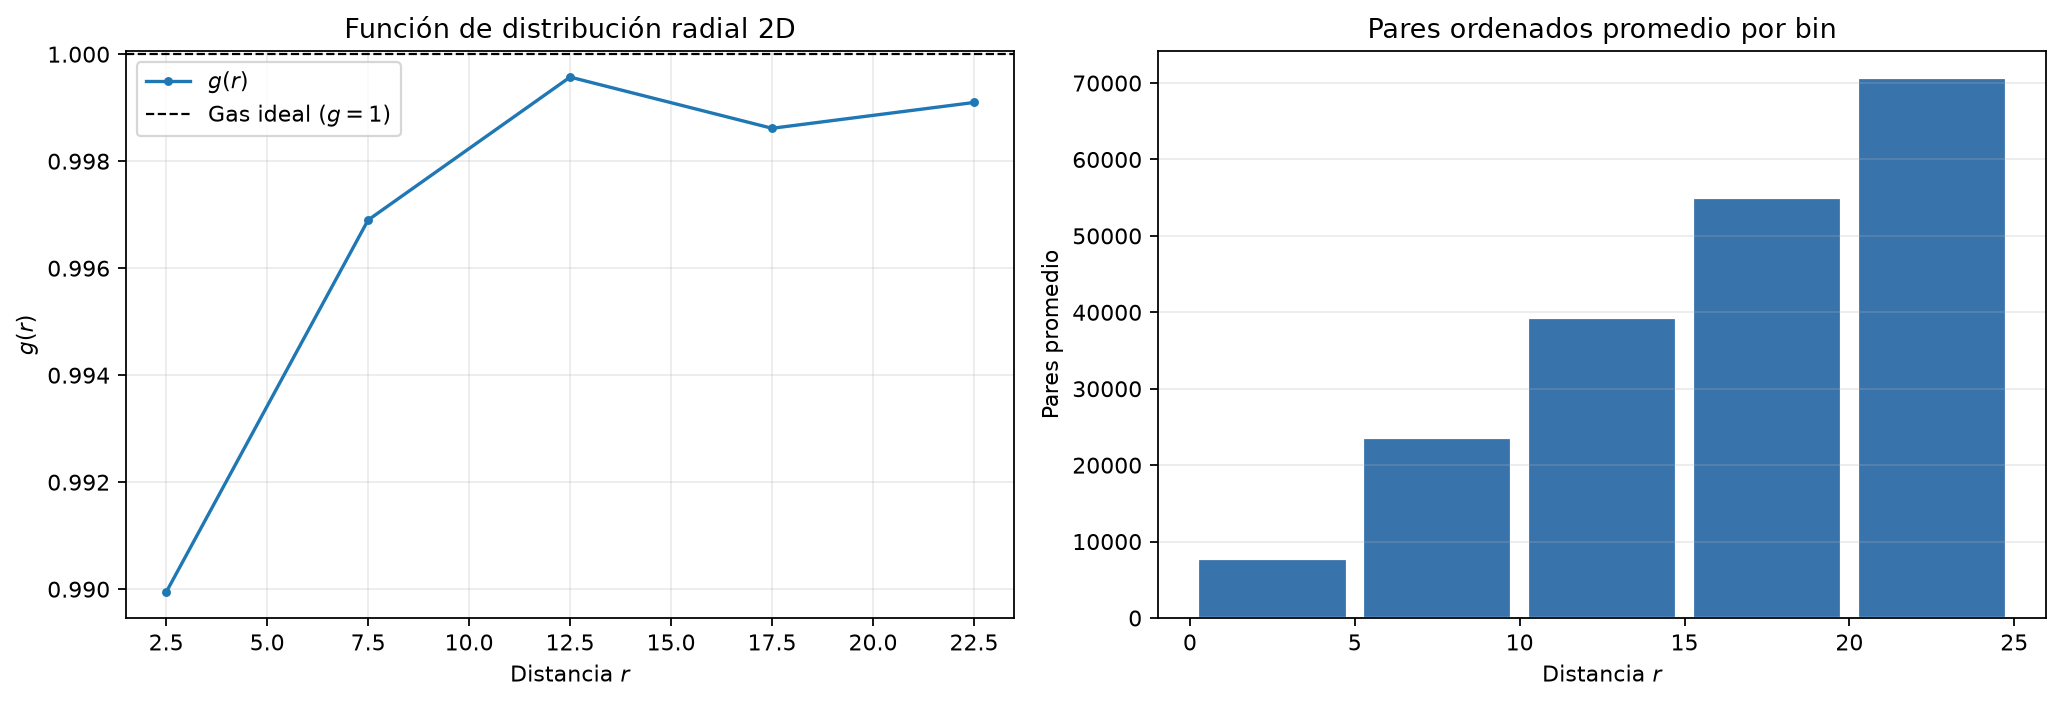
\includegraphics[width=0.9\linewidth]{distribucion_radial.png}
        \caption{Función de distribución radial $g(r)$ del fluido de Lennard-Jones con ancho de bin $\Delta r = 0.25$.}
    \end{figure}


\end{multicols}

%%%%%%%%%%%%%%%%%%%%%%%%%%%%%%%%%


\section*{Referencias}

\begin{enumerate}
    
    \item \href{https://es.scribd.com/document/140663057/Landau-and-Lifshitz-Course-of-Theoretical-Physics-Vol-10-Physical-Kinetics}{Landau \& Lifshitz -- Vol. 10 -- Physical-Kinetics.}
    
\end{enumerate}

\end{document}
